%# -*- coding:utf-8 -*-
%!TEX root = ../thesis.tex



\chapter{控制导向的水下机器人模型建立}
% P86-P115
\label{chap:modelingforcontrol}
% 4.1 引言
% 4.2 控制导向的数学模型
% 4.3 鱼雷型机器人的模型建立
% 4.4 复杂外形机器人的模型建立
% 4.5 计算结果与分析
% 4.6 本章小结
\section{引言 }
水下机器人的模型用来解释本体运动与施加在本体上的力、力矩之间的关系,该模型对于控制和导航都具有重要作用。水下机器人系统需要进行水下航行来验证系统的可行性。然而,用于描述水下机器人动力学特征的数学模型并非完全适用于水下机器人的控制系统设计。动力学、运动学理论常常被用来分析水下机器人的运动,这种方法可以帮助研究者从数学原理的角度对运载器的本体的系统行为有个理性认识。非线性模型识别是基于实验数据对水下机器人系统进行动力学模型参数的估计。研究人员会基于固有的知识,如已经建立的模型,或者使用室内水池实验提取的测试数据,进行水下机器人的探索和系统辨识。然而,数学描述法和系统辨识方法建立的模型主要是为了研究系统行为,而水池实验所需要的成本较高,需要对水下机器人模型有个深度的了解。这些特点都对于水下机器人的控制器设计带来挑战。

合适的控制器对水下机器人成功地进行水下航行与执行任务非常关键。控制器主要分为无模型控制和有模型控制。无模型控制方法能力强大,但是应用该方法训练水下机器人在未知环境中航行需要花费较多的时间进行调节参数,以及无法保证控制器的鲁棒性和自适应性。鲁棒自适应控制方法可以应对水下机器人在适应未知环境中工作时参数变化,稳定地应对一定形式的干扰。因此需要进行用于控制导向的水下机器人模型构建方法研究。

用于鲁棒控制的水下机器人模型建立方法受到了研究者的关注。Yang和Clement等对于小型AUV的运动特点进行研究,分析了水下机器人动力学模型中各项的重要性,并使用数值分析方法为鲁棒补偿器控制建立的水下机器人模型\cite{yang2015modeling}。该方法是基于水下机器人的CAD模型进行数值分析的,并与实验进行对比。虽然数值分析方法可以提供精确度较高的模型,但是其计算量大,且对控制器设计带来一定的流体分析挑战。基于经验数据而对水下机器人模型进行估算也是一个有效且快速的方法,该方法仅仅需要ROV的有关尺寸参数就可以进行ROV模型构建,其中刚度模型质量矩阵也可以采用CAD软件进行测量获得。相比于数值分析法,该方法计算快速,便于编译成一个计算程序,这对于水下机器人的控制器设计很有益。数值分析法和经验法都是可以基于水下机器人的外形进行建模,建立的模型可以适用于非初等几何形状的运载器控制,结合自适应估计部分则可以加强机器人的水下自适应性。具有非初等几何形状的机器人主要是ROV,而与之相比,AUV有很好的流线型,AUV的模型可以参考潜艇模型或者使用系统辨识方法获得模型,但是AUV的数学模型需要进行数学简化方可适用于水下机器人。一般而言,非线性模型的简化是粗略地忽略一些变量,这种方法忽视了各种量的相关性,会给系统控制带来干扰。本部分介绍了一种基于泰勒公式展开的方法,可以将复杂的非线性模型简化为适用于自适应控制的简化模型。


\section{非初等几何外形的水下机器人模型建立}

水下机器人根据流体力学的分布情况,分为流线型的和非流线型的水下机器人。流线型水下机器人的建模多参考潜艇模型简化建立用于控制的模型。非流线型的水下机器人因形状复杂而具有较多的非初等集合外形。在本节中,将介绍具有初等几何外形的水下机器人的建模方法:一种是经验法,另外一种是流体力学软件计算法\cite{eidsvik2015identification,elgenes2017underwater}。两种方法都可以用来计算ROV的模型,并将模型用于控制器设计。

\subsection{经验法}

本节中,将介绍一种估算水下机器人ROV的典型流体动力学参数的方法。估算ROV的流体动力学的参数,应包括质量项,阻尼项,恢复力项。该方法可以用于对多种形状的ROV机器人进行建模,包括作业型ROV和观测型ROV。估计法是基于经验并对实验数据进行分析而总结的一个方法,该方法可以用于不同形状的ROV模型分析\cite{bertram2012practical}。当要采用这种方法对水下机器人进行模型快速估算时,可以保证有相当高的精度。此外,该方法也不需要对ROV模型有很深的了解。在本部分的进一步工作中,由于刚体质量矩阵的系数可以非常容易地从CAD绘图或估计中获得,在本节中进行的这些参数的介绍较少。本节的研究重点将是更难以获得的附加质量和阻尼系数。

\subsubsection{质量项}
质量矩阵中的项是很简单的几何量。如果水下机器人的CAD模型存在,就很容易获得这些项的数值。如果一个CAD模型并不存在,那个这些系数则需要采用积分和平行轴线理论来求取。在进行估计是,假设ROV质量为$m$ [kg]。

在计算与平动有关项时,假设质量是在ROV整个体积内平均分布的。因为ROV在空气中的重量是已知的,因此平动项也可以获得,即,$M_{11} = m$  [kg], $M_{22} = m$ [kg], $M_{33}=m$ [kg]。

旋转自由度系数被定义为力矩和惯性的乘积。对角线上的项称为惯性力矩,其可以由如下公式计算:

\begin{equation}
I_p =  \int_{V}\rho \left ( r \right )\ast r^{2}dV = m \ast r^{2}
\label{eq:chap4:mass}
\end{equation}

假设ROV是矩形体,这样可以得到水下机器人ROV的各个轴的惯性转矩如下:

\begin{equation}
\begin{aligned}
I_4 &= \frac{m}{12}\left ( W^2 + H^2 \right ) \\
    &= \frac{m[kg]}{12}\left ( (W[m])^2 + (H[m])^2) \right )\\
    &= I_4[kgm^{2}] \\
I_5 &= \frac{m}{12}\left ( L^2 + H^2 \right ) \\
    &= \frac{m[kg]}{12}\left ( (L[m])^2 + (H[m])^2) \right )\\
    &= I_5[kgm^{2}]\\
I_6 &= \frac{m}{12}\left ( W^2 + L^2 \right ) \\
    &= \frac{m[kg]}{12}\left ( (W[m])^2 + (L[m])^2) \right )\\
    &= I_6[kgm^{2}]
\end{aligned}
\label{eq:chap4:massrot}
\end{equation}

因假设水下机器人是纯矩形的,那么水下机器人的重心就和几何重心重合,那么其他的不在对角线上的耦合惯性转矩是为零的。

\subsubsection{恢复力}

对于水下机器人而言,当水下机器人本体完全没入到水中时,浮力常常是略大于重力的。这样设计是为了确保,当水下机器人在运行时出现能源中断(耗尽)以及别的系统故障时,水下机器人能够重新浮出水面,而不至于丢失。然而,这个净浮力相比于水下机器人的本体重力往往是比较小,因此在本文进行力平衡分析时候,可以忽略。图\ref{fig:chap4:F1} 是俯仰自由度的恢复力的物理原理图\cite{eidsvik2015identification}。 同理,也可以进行横滚自由度的恢复力分析。

\begin{figure}
\label{fig:chap4:F1}
\centering
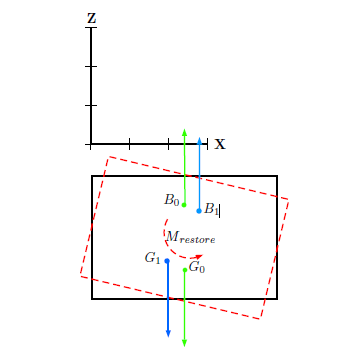
\includegraphics[width = 6cm]{figure/chap4/restoring.png}
\bicaption[fig:chap4:F1]{恢复力原理示意图}{恢复力原理示意图}{Fig.}{Restoring moment concept}
\end{figure}

使用三角法,很容易找到横滚自由度和俯仰自由度的恢复力矩。因为本体上的重心和浮心之间距离是固定的,所以恢复力矩只与浮力和重力之间的力臂长度有关。

如前面所述,ROV在设计的时候往往会让浮力略大于重力,使之具有正浮性。在进行恢复力分析时,是假设重力是等于浮力的,因此重力矢量和浮力矢量之间的力臂长度才是最重要的参数。要估计恢复力矩的大小,就要确定出力臂的长度,但是一般而言,力臂长度很难被估计出来。使用一些CAD软件例如CATIA、 HydroD可以帮助研究者快速的确定重心和浮心的位置。而使用经验法进行估计水动力学参数时,假设浮心的位置是已知的。如此,可以获得ROV的横滚自由度和俯仰自由度的恢复力的公式如下:

\begin{equation}
\begin{aligned}
C_{44} &= -(z_g \ast W-z_b \ast B)\ast cos(\theta) sin(\varphi) \approx W \ast \overline{BG} \ast 1 \ast \varphi \\
C_{55} &= -(z_g \ast W - z_b \ast B) \ast cos(\varphi) sin(\theta) \approx W \ast \overline{BG} \ast 1 \ast \theta\\
B &= W = m \ast G = 9.81 \ast m [N]\\
\label{eq:chap4:restor}
\end{aligned}
\end{equation}
其中,$\overline{BG}$ 是重心和浮心之间的垂直距离。

如果$z_{g}$为零,并且ROV的俯仰与横滚满足小角度理论,那么可以将公式重写如下:

\begin{equation}
\begin{aligned}
C_{44} &\approx (9.81 \ast m) \ast \overline{OB}  \ast \varphi [Nm]\\
C_{55} &\approx (9.81 \ast m) \ast \overline{OB}  \ast \theta [Nm]\\
\end{aligned}
\end{equation}
其中,$\overline{OB}$ 是旋转中心到浮力的距离。

\subsubsection{附加质量}

为了估算ROV的附加质量,就需要使用分析数据。有很多的数据源可以使用,但是在使用这些数据源时候必须采用DNV标准\cite{DNVStard}。DNV标准中采用矩形体的其中两个面作为参考。该假设对于本论文中的ROV是可以适用的,因为所有的ROV都有近似的高度和宽度。高度和宽度的平均值将可以被用来求解估计数据。

因为参考值中假设ROV是矩形体,但是ROV并不是完全的实体,ROV中会有空隙,也会存在渗透流。这个影响可以通过使用一个缩放系数$C_{p}^{mn}$ 对参考值进行校正。该系数是用上标平面内的投影面积除以参考矩形体的平行面的面积而求取。在表\ref{tab:chap4:table1}中列出了用于获得相关投影面积系数的局部坐标系\cite{bertram2012practical}。

\begin{table}
\centering
\label{tab:chap4:table1}
\bicaption[tab:chap4:table1]{投影面积所对应的系数上标}{投影面积所对应的系数上标}{Table}{Projected area coefficient superscript}
\begin{tabular}{cccc}
\toprule
 DOF            & m & n & o\\
\midrule
 Surge \& roll  & X  &Y   &Z   \\
 Sway  \& pitch &  Y &Z   &X   \\
 Heave \& yaw   &Z   &X   &Y   \\
\bottomrule
\end{tabular}
\end{table}

根据DNV标准\cite{DNVStard},矩形体的附加质量的数据如表\ref{tab:chap4:table2}所示。

\begin{table}
\centering
\label{tab:chap4:table2}
\bicaption[tab:chap4:table2]{附加质量系数}{附加质量系数}{Table}{Added mass coefficients}
\begin{tabular}{cccc}
\toprule
 Body shape  & Dimensions(B/A) & Added mass coefficient\\
\midrule
\multirow{7}{4cm}{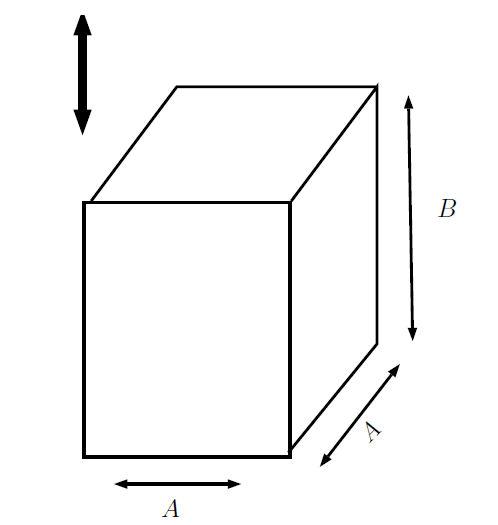
\includegraphics[width = 4cm]{figure/chap4/T2_f.png}}
 & 1.0   &0.68    \\
 & 2.0   &0.36    \\
 & 3.0   &0.24    \\
 & 4.0   &0.19    \\
 & 5.0   &0.15    \\
 & 6.0   &0.13    \\
 & 7.0   &0.08    \\
\bottomrule
\end{tabular}
\end{table}


对于旋转自由度,没有找到经验3D数据。 不同的
因此必须使用方法。 使用类似形状的知识之一
知道球体(3D)的附加质量差异和无限长的差异
相同半径(2D)的圆柱体为50%\cite{bertram2012practical}。 通过将这个关系转换成问题
手头可以创建一个旋转自由度的程序。

对于水下机器人的旋转自由度,并没有找到3D经验数据。因此必须采用不同的方法来进行分析。可以通过找不同形状的附加质量之间的相似性,来研究附加质量之间的关系,例如,相同直径的三维球体和无限长的二维圆柱体的附加质量相差50$\%$。通过将这种关系转成手头可以处理的问题,就有可能创造出一个旋转自由度的附加质量求解程序。

求解程序如下:
步骤一:使用经验3D数据找到平动自由度的附加质量;
步骤二:使用2D数据和切片理论确定平动自由度的附加质量;
步骤三:使用缩放系数对比两种方法的不同;
步骤四:使用2D数据和切片理论找到旋转自由度的附加质量;
步骤五:对结果进行调整。

通过使用以上流程,就有可能找到附加质量矩阵对角线上的所有项。

为了利用好参考的经验数据, 一个合适的缩放程序就需要考虑ROV和参考的矩形体之间的差异。有很多种方法可以用来处理这个差异,但是在众多的方法中能够对所有的量都能做到获取便捷才是最佳的选择。在本文中,附加值质量系数是使用投影面积进行缩放调整的。投影面积可以使用CAD软件如CATIA获取,分别测量出三个平面的投影面积。此外,也可以手动地测量估算出来ROV在三个平面的投影面积。这个投影面积然后被用来计算系数$C_{p}^{mn}$。因此,可以得到三个平面的系数计算公式如下:

\begin{equation}
\begin{aligned}
C_{p}^{XY} = \frac{A_{p}^{XY}}{A} = \frac{A_{p}^{XY}}{L \ast W} \\
C_{p}^{YZ} = \frac{A_{p}^{YZ}}{A} = \frac{A_{p}^{YZ}}{H \ast W} \\
C_{p}^{ZX} = \frac{A_{p}^{ZX}}{A} = \frac{A_{p}^{ZX}}{L \ast H} \\
\end{aligned}
\end{equation}

对于平移运动的附加质量,往往首先是对纵荡运动进行分析。通过观察表,可以发现$\frac{B}{A}$的最小值为1.0。这也就意味着只有水下机器人的长度尺寸大于宽度和高度尺寸时候,参考的数据才是有效的。这个要求对于大多数的水下机器人都是成立的。

第一步是为$A_{11}$找到相应的经验3D系数。 查询表格值需要确定出ROV的高度与宽度。 因为表格仅包含给定数量的数据点
($\frac{b}{a}$)值,对于数据集在这两数据点之间的情况就需要进行线性化差值。

数据点之间的距离线性化是采用如下公式来计算经验值:

\begin{equation}
\begin{aligned}
C_a(\frac{b}{a}) = \frac{C_a(2)-C_a(1)}{X_2 - X_1} \ast  (X - X_2) + C_a(2)
\end{aligned}
\end{equation}

然后,需要计算参考体积:

\begin{equation}
\begin{aligned}
V_R = b \ast a^2
\end{aligned}
\end{equation}

修正后的附加质量公式如下:

\begin{equation}
\begin{aligned}
A_{ij} = C_a V_R \rho_{water}(C_p^{no})^2(C_p^{mo})^(C_p^{mn})
\end{aligned}
\end{equation}

这样,$A_{11}$ 就可以使用3D数据进行计算并给出一个相对合理的估计。

同样地,其余的附加质量系数也可以采用切片理论并参考2D的系数和DNV标准进行估算。第一步就是确定宽度与高度的关系。然后,将宽高比的数值带入到方程中来获得附加质量系数。当使用切片理论时,需要计算参考面积而不是参考体积:

\begin{equation}
\begin{aligned}
A_R = \pi \ast (a)^{2}
\end{aligned}
\end{equation}

这样,就可以得到纵荡自由度的2D附加质量系数:
\begin{equation}
\begin{aligned}
A_{11}^{2D} = \rho \ast C_a A_r(C_p^{no})^2(C_p^{mo})(C_p^mn)
\end{aligned}
\end{equation}

通过应用切片理论,对2D的附加质量进行积分,可以获得3D附加质量如下:

\begin{equation}
\begin{aligned}
A_{11} = \int_{L/2}^{-L/2}A_{11}^{2D}dx
\end{aligned}
\end{equation}

这样就可以找到切片理论和3D计算之间差异:

\begin{equation}
\begin{aligned}
\lambda = \frac{A_{11}^{empirical-3D}}{A_{11}^{strip-3D}}
\end{aligned}
\end{equation}
缩放系数$\lambda$ 给出了两个方法之间的关系。因此显而易见的是,如果这种关系对于所有自由度都是有效的,则可以使用切片理论计算附加质量,然后缩放以获得正确的附加质量估计值。

对于旋转自由度,也可以采用和平移自由度内类似的方法,使用缩放系数对切片理论计算的结果进行调整。2D的附加质量系数可以从DNV的有关标准中查阅。旋转自由度的2D附加质量的一般公式为
\begin{equation}
\begin{aligned}
A_{ii}^{2D} = \rho \ast C_a \ast \pi a^4 (C_p^{no})(C_p^{mo})(C_p^{mn})
\end{aligned}
\end{equation}

在整个长度上进行积分,可以得到

\begin{equation}
\begin{aligned}
A_{ii}^{'} = \int_{(L,B,H)/2}^{-(L,B,H)/2}A_{ii}^{2D}dx
\end{aligned}
\end{equation}

最近进行缩放调整,就可以得到旋转自由度的附加质量系数:

\begin{equation}
\begin{aligned}
A_{ii} = A_{ii}^{'} \lambda [kgm^{2}]
\end{aligned}
\end{equation}

\subsubsection{阻尼力}

ROV的阻尼力是和机器人的运行速度有关的。如果阻尼是高度非线性的,就很难对其进行准确地估计。

为了分析水下机器人的阻尼,就必须对阻尼的概念有所介绍。第二章在水下机器人的模型部分介绍了一些相关知识。ROV受到阻尼主要包括线性和二次摩擦阻尼以及由于旋涡脱落而产生的相关阻尼。由于旋涡脱落而产生的阻尼可以建模为二阶方程(莫里斯方程)。这样ROV受到的阻尼主要可以使用线性和二阶阻尼的合系数来描述其作用大小。

\begin{equation}
\begin{aligned}
B = B ^{LIN} + B ^{NL}
\end{aligned}
\end{equation}
其中,$B ^{LIN}$是线性阻尼系数,$B ^{NL}$是非线性阻尼系数。

线性阻尼部分包括线性摩擦阻尼;而非线性阻尼则包括了所有的高阶阻尼项,例如湍流摩擦阻尼和旋涡脱落而产生的阻尼。对于低速航行的ROV,由于湍流和漩涡而产生的阻尼作用小,线性阻尼会是主要的部分。同样,高速航行的水下机器人中,非线性阻尼会起主要的作用。因此,显而易见的是,两种阻尼对于描述ROV在整个运行阶段中的阻尼行为都是至关重要的。

如前所述,二次阻尼表示所有高阶阻尼的贡献,但主要是涡旋脱落和湍流边界层表皮摩擦。 可能从线性阻尼开始更符合逻辑,但是对于经验性的角度来说,利用Morison方程估计二次阻尼更容易。 使用势能理论并不能求得二次阻尼,因为势能理论假定水是无旋转的,不可压缩的和无粘性的流体。 这种假设对于许多应用来说是足够的,但是当涉及阻尼时,就必须考虑水的粘度的作用。

正如附加质量一样,唯一可用的3D参数是纵荡自由度的3D阻力系数,并且这里仍然假定ROV的长度大于宽度和高度。因此,估计步骤类似于附加质量。二次阻尼将使用3D系数估算,然后使用Morison方程进行估算。 将估算的结果进行缩放,然后再将相同的缩放数量应用于剩余自由度里。如前所述,阻力系数是纯粹用于描述特定几何形状的粘滞阻力的经验系数。由于ROV的尺寸已知,因此可以通过查询相关文献找到3D和2D阻力系数\cite{eidsvik2015identification,bertram2012practical}。

应当指出阻尼系数的公式如下:

\begin{equation}
\begin{aligned}
C_D = \frac{F_D}{\frac{1}{2}\rho \ast A \ast u \left | u \right |}
\end{aligned}
\end{equation}

平移运动的二次阻尼系数可以使用莫里斯方程得到,公式如下:

\begin{equation}
\begin{aligned}
B_{jj}^{NL}v_j|v_j| = \frac{\rho}{2}C_D A v_j |v_j| \lambda(C_p^{no}), j = 1,2,3
\end{aligned}
\end{equation}

需要注意的是莫里斯方程里的参考面积是使用投影面积进行缩放调整得到。2D的切片理论和3D的阻尼系数的差异需要被计算出来。对莫里斯方程的所有必要的术语进行修正,就可以计算出平移自由度阻尼。

\begin{figure}
\label{fig:chap4:F2}
\centering
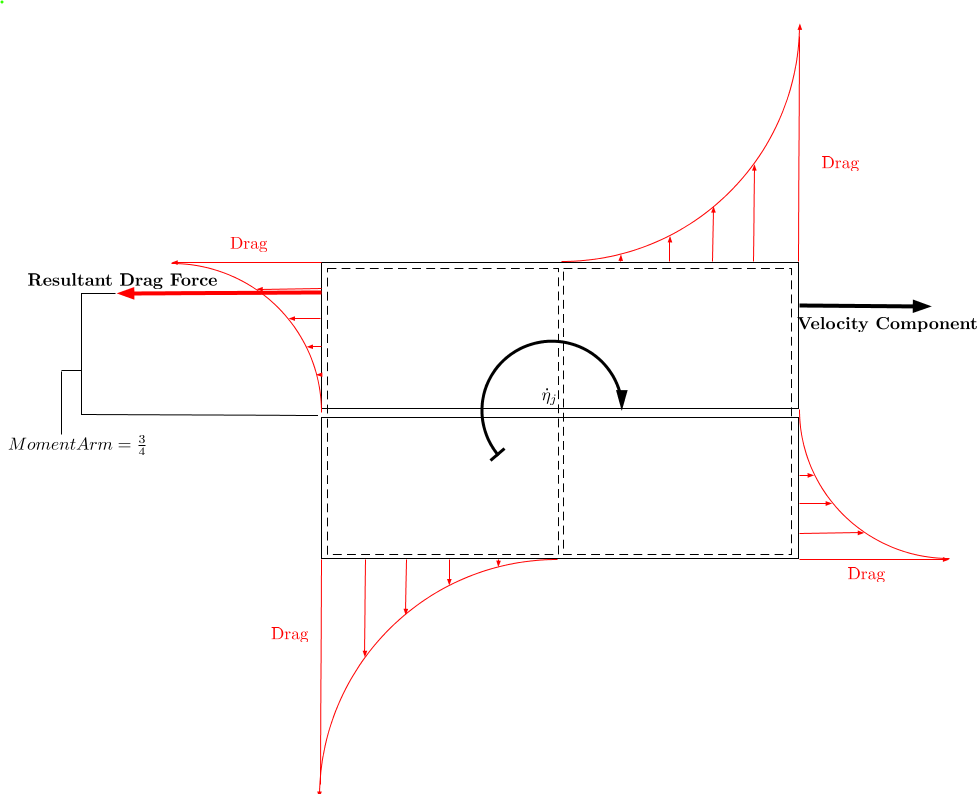
\includegraphics[width = 12cm]{figure/chap4/ROV_disc.jpg}
\bicaption[fig:chap4:F2]{ROV的阻尼力离散}{ROV的阻尼力离散}{Fig.}{Discretization of ROV damping\cite{eidsvik2015identification}}
\end{figure}

要估计旋转自由度中的非线性阻尼是相当具有挑战性的,主要是因为没有好的经验方法。 由于作者并不能够从别的资料找到一种可靠的方法来估计旋转自由度的非线性阻尼,就必须建立一种新方法来进行估算。这种方法建立在这个事实上,即小旋转可以将旋转运动等价为平移运动。

首先将ROV划分为围绕每个轴的总共4个象限(将所有3个轴共计加上12个象限)。此外,将假设每个象限仅在水平或垂直方向上移动。 通过查看图\ref{fig:chap4:F2},这意味着固体象限将水平移动,装订的象限将垂直移动。这里,最重要的假设是象限具有小角度旋转。

因为二次阻尼是相对于速度的二次函数,在象限靠近中心的位置阻尼为零,而在最外面则阻尼最大,可以参考图\ref{fig:chap4:F2}。力矩的力臂大约在象限内远离旋转中心中的$\frac{3}{4}$的位置处。旋转阻尼可以由每个象限的阻尼系数和局部的末端的平移速度来表示。

要表示旋转运动的阻尼,首先要确定不同象限的平移速度,不同自由度的平移速度表示如下:

\begin{equation}
\begin{aligned}
\overline{v_2} [m/s] = v_2 [rad/s] \ast \frac{(L/B/H)}{2}[m]
\end{aligned}
\end{equation}

每个象限的阻尼力系数需要查询文献论文中的表格\cite{eidsvik2015identification}。每个象限的阻尼力公式可以写为($om$ 是水平象限,$mn$是垂直象限):
\begin{equation}
\begin{aligned}
F_{quadrant}^{j} = \frac{1}{2} \ast \frac{1}{3} \ast \rho \ast C_D \ast A \ast  C_p^{om/mn} \ast  \lambda \overline{v_2} \ast | \overline{v_2}|, j = 4, 5, 6
\end{aligned}
\end{equation}

将每个象限的力乘以力臂就可以得到绕轴的力矩:


\begin{equation}
\begin{aligned}
 \overline{M}_{quad}^j= F_{quadrant}^{j} \ast \frac{3}{4} \frac{L,B,H}{2}
\end{aligned}
\end{equation}

再次说明的是,L,B或H取决于自由度以及它是否是水平的或垂直象限。

这样可以得到水平的速度:

\begin{equation}
\begin{aligned}
M_{quad}^{j} = \overline{M}_{quad}^{j} \ast (\frac{L,B,H}{2}) ^2
\end{aligned}
\end{equation}

将水平和垂直象限的阻尼加到一起就可以得到合阻尼力矩如下:

\begin{equation}
\begin{aligned}
M_{tot} = 2 \ast M_{quad-Horizontal}^{j}  + 2 \ast M_{quad-Vertical}^{j}
\end{aligned}
\end{equation}

对于线性阻尼,是很难进行分析估计的。虽然有很多的水面船的近似估计存在。对于水面船的线性摩擦阻尼,Fossen提出如下的经验公式:

\begin{equation}
\begin{aligned}
B_{11}^{LIN} &= \frac{M_{11} + A_{11}}{T_{surge}} \\
B_{22}^{LIN} &= \frac{M_{22} + A_{22}}{T_{sway}} \\
B_{33}^{LIN} &= 2 \Delta \zeta_{heave} \omega_{heave} [M_{33} + A_{33}(\omega_{heave})]\\
B_{44}^{LIN} &= 2 \Delta \zeta_{roll} \omega_{roll} [I_{44} + A_{44}(\omega_{roll})]\\
B_{55}^{LIN} &= 2 \Delta \zeta_{pitch} \omega_{pitch} [I_{55} + A_{55}(\omega_{pitch})]\\
B_{66}^{LIN} &= \frac{I_{66}+A_{66}}{T_{yaw}}
\end{aligned}
\end{equation}
其中,$T_{DOF} = \frac{T_n(DOF)}{2\Pi \zeta}$, $T_n(DOF)$是每个自由度的自然周期,$\zeta$是阻尼比。
本文中研究的是ROV,但可以采用水面船相类似的方法进行处理。首先,给出一阶粘性阻尼的自由振动方程:

\begin{equation}
\begin{aligned}
(m+m_a)\ddot{\overline{X}} + K_L \dot{\overline{X}} + g \overline{X} = 0
\end{aligned}
\end{equation}

除以ROV的质量并求得状态方程根如下:

\begin{equation}
\begin{aligned}
\left \{ \begin{matrix}
\lambda _1 \\
\lambda _2
\end{matrix} \right \}
=  - \frac{K_L}{2m}\pm \sqrt{K_L^2 - 4mg}
\end{aligned}
\end{equation}

那么可以得到临界阻尼为$K_{L} = 2m\omega_n$,将临界阻尼带入方程可得:

\begin{equation}
\begin{aligned}
\ddot{\overline{X}} + 2\zeta \omega_n \dot{\overline{X}} + \omega_n^2 \overline{X} = 0
\end{aligned}
\end{equation}
其中,
\begin{equation}
\zeta = \frac{K_L}{K_{L,critical}} = \frac{K_L}{2m\omega_n}
\end{equation}
这样就可以使用三个参数来估计线性阻尼。质量和自然频率可以被计算,但是阻尼比需要预先设定一个值。对于水面船,横滚自由度的阻尼比一般的范围是$2-10\%$。而对于ROV,阻尼比可设定为$2.5\%$。虽然这个阻尼比的值不能确定完全准确的值,但是它是在一个相对合理的范围内。

自然频率给出如下:

\begin{equation}
\begin{aligned}
\omega_n =  \sqrt{\frac{g}{m+m_a}}
\end{aligned}
\end{equation}

线性阻尼可得:
\begin{equation}
\begin{aligned}
K_L = 2 \zeta m \sqrt{\frac{g}{m+m_a}}
\end{aligned}
\end{equation}

由于恢复力的存在,线性阻尼在横滚和俯仰自由度内可使用这种方法来计算。假设俯仰自由度内,线性阻尼和二次阻尼的系数间存在一种比例关系,那么可使用缩放系数来从俯仰或者横滚自由度来获得偏航的阻尼。对于平移自由度缩放系数是0.16。

将上面的线性和非线性阻尼项加上一起就可以获得ROV的完全阻尼矩阵的估计。

\subsection{基于CFD的数值计算法}

本节中,将介绍一种使用流体数值计算软件来给水下机器人进行建模的方法。在前的一部分中,已经介绍了非初等几何类型的ROV的经验分析法,在本节中,所有的模型关键项都是基于CAD的模型已知的。刚体惯性质量矩阵可以使用CAD软件如CATIA进行测量,恢复力主要是在确定水下机器人的浮心和重心后,参考第二章水下机器人模型中对恢复力的定义确定。本节主要集中于使用CFD软件对附加质量和阻尼力项进行计算上。

\subsubsection{附加质量}

水下机器人形状会给附加质量带来影响,对于复杂形状的水下机器人,采用基本形状的船体进行预测和逼近的经验公式往往是不准确的。为了解决这个问题,使用WAMIT和AWQA软件可以计算水下机器人的附加质量项。在本文例子中,首先使用WAMIT的计算值作为对比,而使用AWQA海洋工程计算软件来完成对附加质量项的估计。

首先使用流体计算软件计算一个球体的附加质量,球体的附加质量的理论值为$2/3\pi \rho r^3$。球体的附加质量的理论值可以用来验证流体软件中计算附加质量的配置是否正确,计算的对比结果如表\ref{tab:chap4:table3-1},其中球体的直径为1m,密度为1kg/m3,水深为10m。

要计算水下机器人的附加质量,首先对水下机器人的模型进行简化预处理,以保证AQWA软件计算的质量和效率。AWQA是集成在ANSYS中的一款通用的流体动力学分析软件,可以使用ANSYS的网格预处理MESH模块建立网格,网格设计不要太密,也不要太少。网格太少会让计算的结果可行度降低,网格太密又会让计算时间很长,导致计算积累误差出现,计算的结果可信度也会降低。图\ref{fig:chap4:F3}显示3000m级别的工作性ROV在AWQA软件里的几何表示图。

\begin{table}
\centering
\label{tab:chap4:table3-1}
\bicaption[tab:chap4:table3-1]{球体附加质量}{球体附加质量}{Table}{Added mass of a sphere}
\begin{tabular}{cccc}
\toprule
           & Theoretical & WAMIT     & AWQA     \\
\midrule
 Surge(kg) & 2.0944      & 2.084236  &2.1406    \\
\bottomrule
\end{tabular}
\end{table}

\begin{figure}
\label{fig:chap4:F3}
\centering
\subfigure[CATIA中模型简化]{
\label{fig:chap4:F3a}
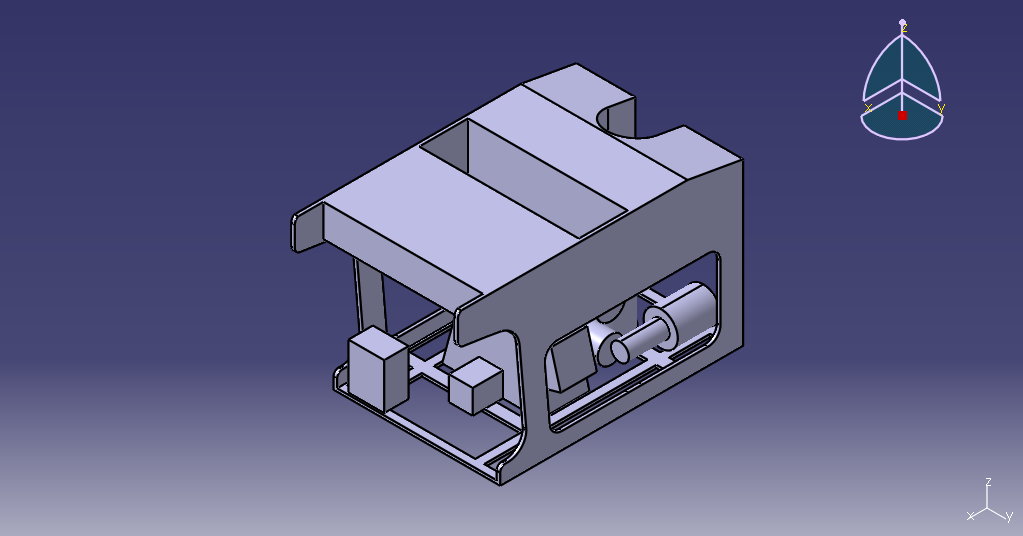
\includegraphics[width = 13cm]{figure/chap4/catia_aqwa.png}
}
\subfigure[AQWA中模型网格]{
\label{fig:chap4:F3b}
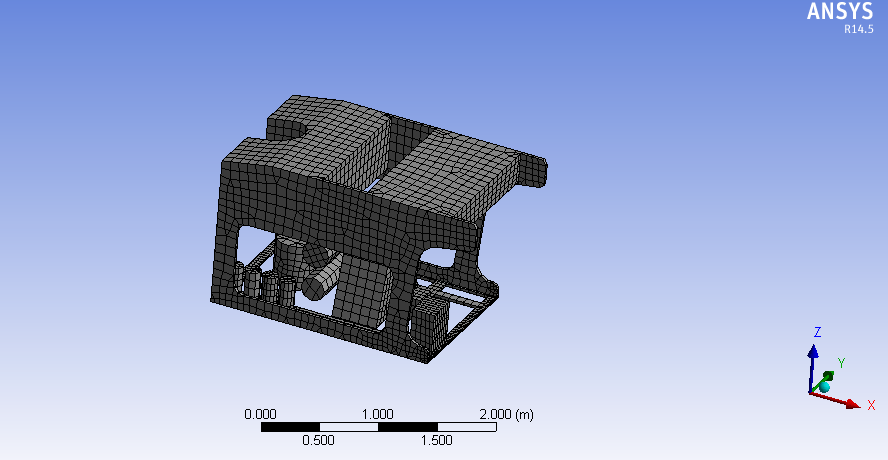
\includegraphics[width = 13cm]{figure/chap4/aqwa_mesh.png}
}
\bicaption[fig:chap4:F3]{ROV简化与网格模型几何表示}{ROV简化与网格模型几何表示}{Fig.}{Geometric representation of ROV in AWQA and CATIA}
\end{figure}


AQWA软件中的设置条件如下:水下机器人为水下5m的水深处,海水密度为1025$kg/m^3$, 水深100m, 水域为正方形($100\times100m$),波浪周期范围为1-125.664秒, 波浪频率范围为0.008-1Hz,波浪方向为水平面内-180-180度且间隔为45度的8个方向, 结合计算机的配置,网格节点数为5468,网格大小范围为15mm-150mm。

由于使用AWQA计算附加质量需要确定刚度质量矩阵,使用CATIA软件可以获得3000m水下机器人的$M_RB$如下:

\begin{equation}
\begin{aligned}
M_{RB} = \begin{bmatrix}
   1468&0   &0   &0&0&0 \\
     0 &1468&0   &0&0&0 \\
     0 &0   &1468&0&0&0 \\
     0 &0   &0   &428.777 &-19.904 &-0.815\\
     0 &0   &0   &-19.904&819.483 &0.473  \\
     0 &0   &0   &-0.815 &0.473   &775.496
         \end{bmatrix}
\end{aligned}
\end{equation}

\subsubsection{阻尼力}

水下机器人受到流体阻尼力主要分为线性阻尼和非线性阻尼。两种阻尼都和水下机器人的运行速度有关,由于水下机器人运行的速度范围内两种阻尼都存在,为了精确地估计水下机器人受到的阻尼力,本节选择使用STAR CCM+ 流体计算软件对水下机器人,如3000m级别ROV,进行量化阻尼分析。除了前一节本文介绍的经验估算法,二次阻尼也可以采用如下公式进行粗略的确定阻尼行为。二次阻尼表示如下:

\begin{equation}
\begin{aligned}
f(U)=-\frac{1}{2}\rho_d C_D(R_n)AU|U|
\end{aligned}
\end{equation}
其中,$U$是机器人运行速度,$\rho_{d}$是流体密度,$A$是投影的横截面积,$C_D(R_n)$是阻尼系数,该系数与雷诺数$R_{n}$有关。

本部分是采用CFD流体计算软件进行阻尼分析,但又结合水下机器人建模目的是用于控制的,因此仅需要根据控制目标对ROV的受控自由度进行阻尼分析。采用STAR CCM+流体计算软件对深水ROV模型进行阻尼分析,主要分为纵荡、垂荡、偏航自动度的流体计算的阻尼分析。平移运动如垂荡自由度的阻尼分析设置需给出运行速度范围、网格设置以及边界层设置。

以前进计算为例,在来流方向,计算域取10倍的ROV长度,前端网格长度为ROV的长度的3倍,后端网格长度为ROV长度的7倍;在宽度方向上,整体网格宽度取ROV宽度的5倍;使用STAR CCM+进行网格划分,计算域内的网格模型为TRIM模型,在ROV周围采取加密措施,保证流动细节的捕捉,生成的体网格的数量为332万,网格显示如图\ref{fig:chap4:F4}。边界条件设置:设置入口速度边界,大小为0-1.5m/s,出口设置为压力出口,壁面采用无滑移边界。湍流模型采用Realizable K-Epsilon Two-layer(RKE)模型,边界层处理采用Two-layer all y与wall treatment。湍流强度为0.05,湍流尺度为0.1m,边界层增长率为1.2。上浮计算的例子也与前进的计算例子类似,在高度方向,网格长度是10的ROV长度,网格类型是TRIM,网格数量为330万,在ROV的周围采取加密措施,入口速度大小为0-1m/s。前进计算的速度矢量图和力收敛显示如图\ref{fig:chap4:F5},表示数值计算是成功的。

对于偏航旋转计算,旋转的计算域有两个区域,其中有一个是旋转域,外部区域的长度和宽度一致,为ROV的10倍,中间旋转域直径为ROV的长度1倍,旋转域采用的模型是运动参考坐标系(MRF)。ROV的旋转速度设置为0-1.5rad/s,网格数量为,网格类型为TRIM。边界层设置参考前进计算例子进行设置。
偏航自由度旋转运动的计算域网格如图\ref{fig:chap4:F6}。

\begin{figure}
\label{fig:chap4:F4}
\centering
\subfigure[]{
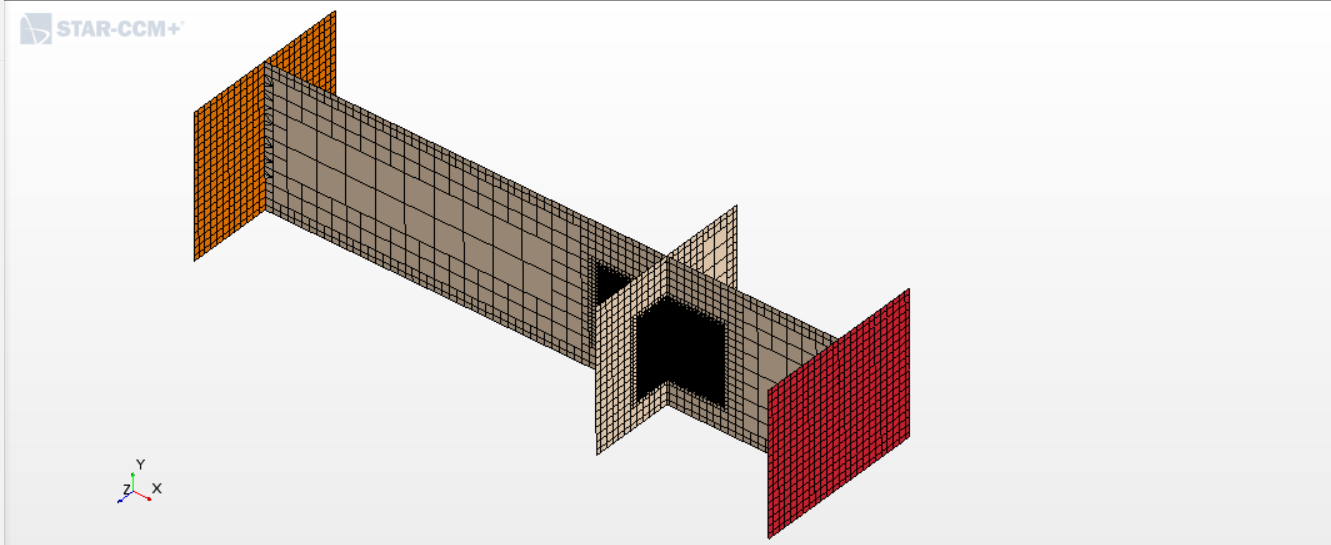
\includegraphics[width = 15cm]{figure/chap4/mesh1.png}
}
\subfigure[]{
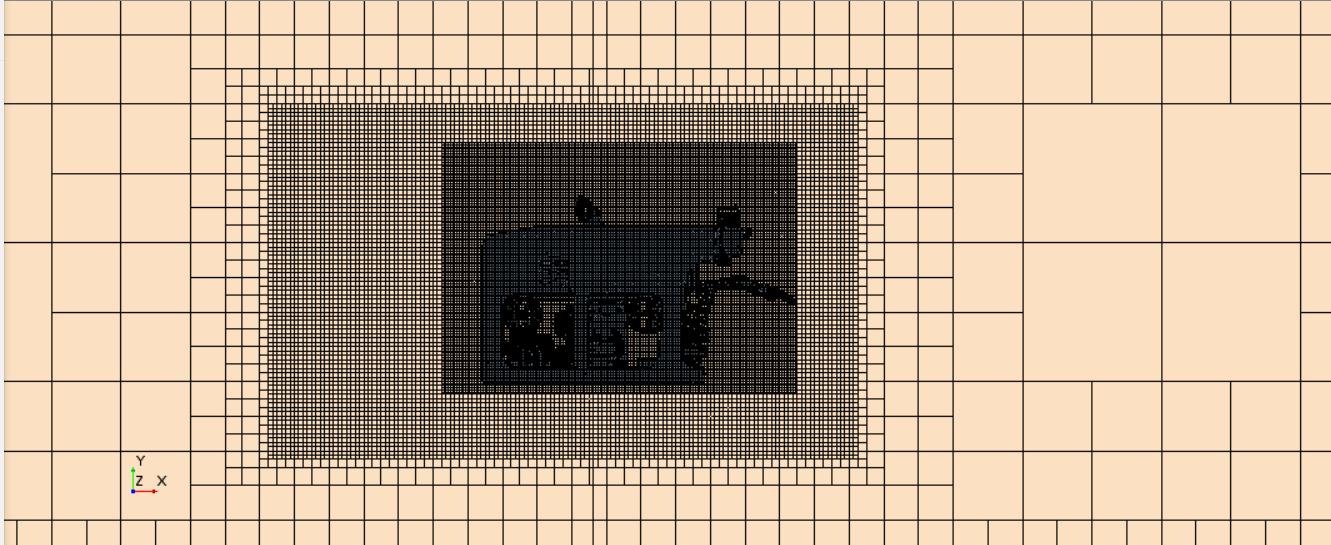
\includegraphics[width = 15cm]{figure/chap4/mesh2.png}
}
\bicaption[fig:chap4:F4]{纵荡运动网格}{纵荡运动网格}{Fig.}{The mesh of ROV surge motion}
\end{figure}

\begin{figure}
\label{fig:chap4:F5}
\centering
\subfigure[]{
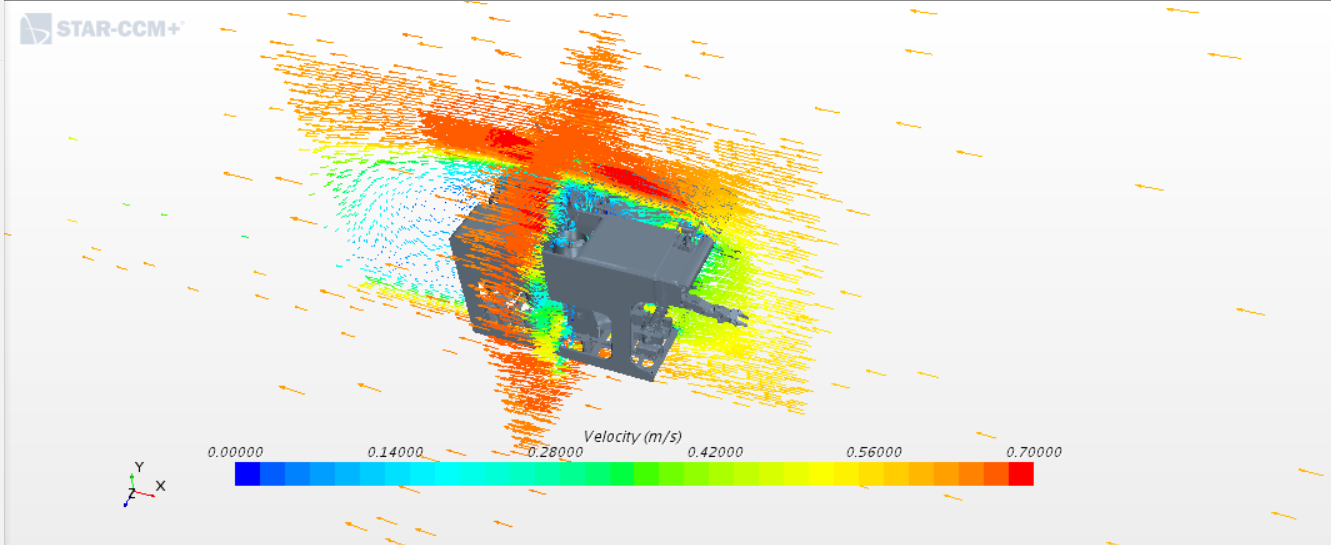
\includegraphics[width = 15cm]{figure/chap4/rov_surge1.png}
}
\subfigure[]{
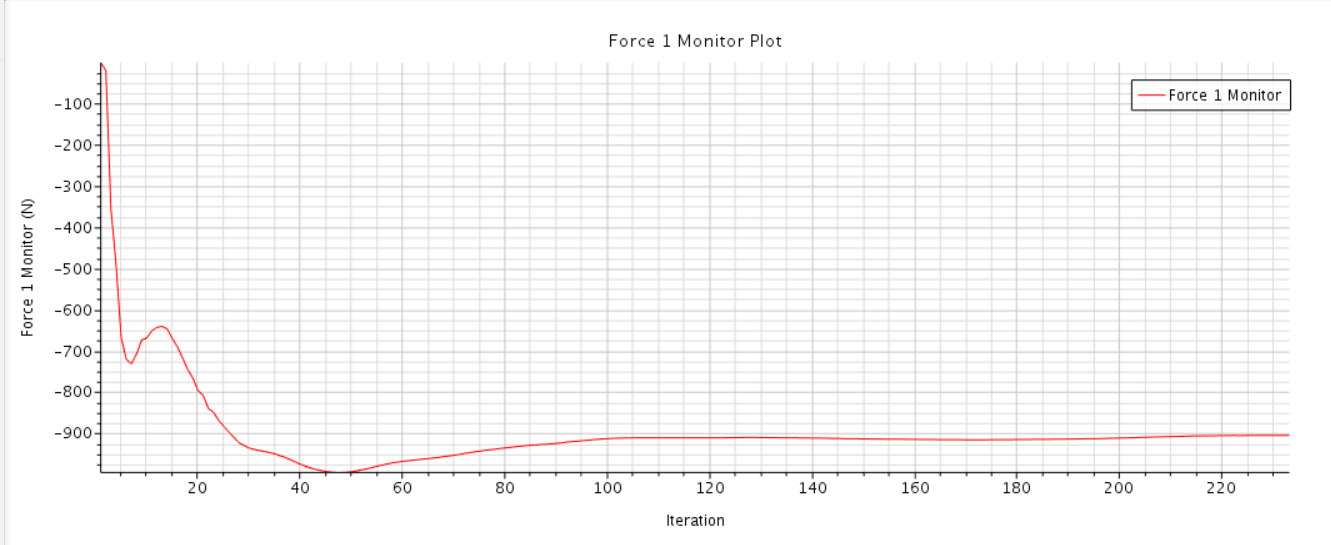
\includegraphics[width = 15cm]{figure/chap4/rov_surge2.png}
}
\bicaption[fig:chap4:F5]{纵荡运动分析与阻力}{纵荡运动分析与阻力}{Fig.}{ROV surge analysis and damping force}
\end{figure}




\begin{figure}
\label{fig:chap4:F6}
\centering
\subfigure[]{
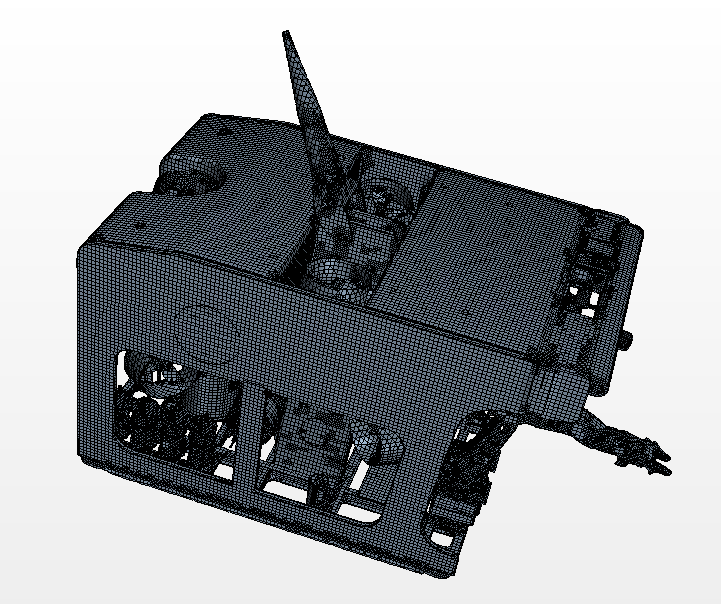
\includegraphics[width = 10cm]{figure/chap4/mesh3.png}
}
\subfigure[]{
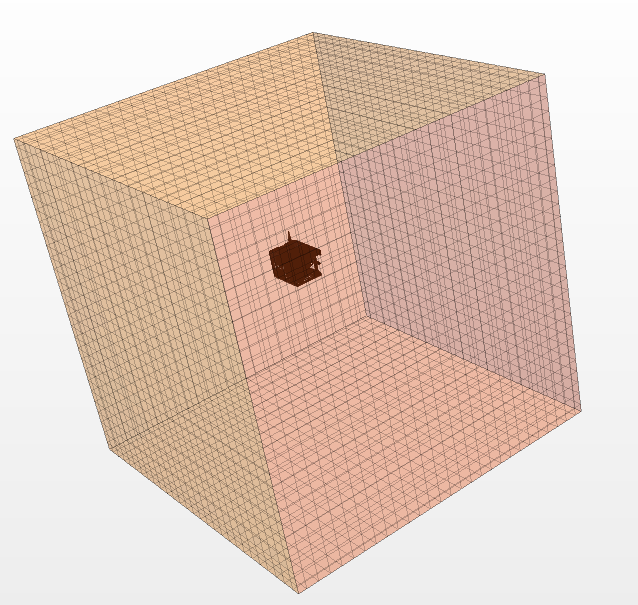
\includegraphics[width = 10cm]{figure/chap4/mesh4.png}
}
\bicaption[fig:chap4:F6]{偏航运动网格}{偏航运动网格}{Fig.}{The mesh of ROV yaw motion}
\end{figure}


\subsection{结果与分析 }

本节首先介绍经验法和流体数值计算方法来估算3000m的深海ROV的模型的流体动力学参数。
经验法相关的参数如下:水下机器人的长度$L=2480[mm]$,高度$H=1630[mm]$,宽度$W=1400[mm]$,水流密度为$1000[kg/m^3]$, 正视图投影面积$PF= 1.92 \times 10^6[mm^2]$,侧视图投影面积$PS= 2.782 \times 10^6[mm^2]$, 上视图投影面积$PT= 2.215\times 10^6[mm^2]$,俯仰和横滚自由度的恢复力系数$C_p = 5697$,线性和非线性的阻尼缩放系数$\lambda = 0.16$。

经过经验法的附加质量和阻尼力计算程序的运行计算,可以得到结果如下:

附加质量项
\begin{equation}
\begin{aligned}
\bm{M_{A}} = \begin{bmatrix}
   1014.070&0   &0   &0&0&0 \\
     0 &2143.288&0   &0&0&0 \\
     0 &0   &1706.464&0&0&0 \\
     0 &0   &0   &242.965 &0 &0\\
     0 &0   &0   &0 & 671.014 &0 \\
     0 &0   &0   &0 &0   &543.627
         \end{bmatrix}
\end{aligned}
\end{equation}

阻尼力项$\bm{D}$包括线性阻尼$\bm{D_L}$和非线性阻尼$\bm{D_N}$,且满足如下公式
\begin{equation}
\begin{aligned}
\bm{D} = \bm{D_L} + \bm{D_N}\nu
\end{aligned}
\end{equation}

线性阻尼项结果
\begin{equation}
\begin{aligned}
\bm{D_L} = \begin{bmatrix}
   148.153&0   &0   &0&0&0 \\
     0 &273.998&0   &0&0&0 \\
     0 &0   &197.270&0&0&0 \\
     0 &0   &0   &97.815 &0 &0\\
     0 &0   &0   &0 & 145.699 &0 \\
     0 &0   &0   &0 &0   &178.869
         \end{bmatrix}
\end{aligned}
\end{equation}

非线性阻尼项结果
\begin{equation}
\begin{aligned}
\bm{D_N} = \begin{bmatrix}
   925.958&0   &0   &0&0&0 \\
     0 &1712.486&0   &0&0&0 \\
     0 &0   &1232.940&0&0&0 \\
     0 &0   &0   &254.366 &0 &0\\
     0 &0   &0   &0 & 652.675 &0 \\
     0 &0   &0   &0 &0   &801.264
         \end{bmatrix}
\end{aligned}
\end{equation}

使用STAR CCM+软件分别对纵荡、垂荡、偏航自由度进行阻尼分析,可以得阻尼力结果如表\ref{tab:chap4:table3-2}、表\ref{tab:chap4:table3-3}和表\ref{tab:chap4:table3-4}所示。计算的纵荡、垂荡速度流线图结果可以见图\ref{fig:chap4:F7}和图\ref{fig:chap4:F8}。图\ref{fig:chap4:F9}给出了偏航旋转运动的矢量图和速度线图。采用二阶多项式来对阻尼力数据进行拟合分别对纵荡、垂荡、偏航三个模式的阻尼力进行拟合,这可以得到速度和阻尼力之间的关系,分别如图\ref{fig:chap4:F10}、图\ref{fig:chap4:F11}和图\ref{fig:chap4:F12}。


\begin{table}
\centering
\label{tab:chap4:table3-2}
\bicaption[tab:chap4:table3-2]{纵荡自由度阻尼分析}{纵荡自由度阻尼分析}{Table}{ROV surge damping}
\begin{tabular}{ccccccc}
\toprule
 Velocity(m/s)    & 0.3 & 0.6 & 0.9 &1.2  &1.5   \\
\midrule
 Damping force(N) & 99.9 &398 &905 & 1610 & 2520  \\
\bottomrule
\end{tabular}
\end{table}

\begin{table}
\centering
\label{tab:chap4:table3-3}
\bicaption[tab:chap4:table3-3]{垂荡自由度阻尼分析}{垂荡自由度阻尼分析}{Table}{ROV heave damping}
\begin{tabular}{ccccc}
\toprule
 Velocity(m/s)    & 0.25   & 0.5 & 0.75    &1     \\
\midrule
 Damping force(N) & 111    & 448 & 1003.56 & 1780 \\
\bottomrule
\end{tabular}
\end{table}

\begin{table}
\centering
\label{tab:chap4:table3-4}
\bicaption[tab:chap4:table3-4]{偏航自由度阻尼分析}{偏航自由度阻尼分析}{Table}{ROV yaw damping}
\begin{tabular}{cccccc}
\toprule
 Velocity(rad/s)    & 0.3   & 0.6 & 0.9  &1.2   & 1.5   \\
\midrule
 Damping torque(Nm) & 142.4 & 633 & 1392 & 2442 &3958    \\
\bottomrule
\end{tabular}
\end{table}

\begin{figure}
\label{fig:chap4:F7}
\centering
\subfigure[]{
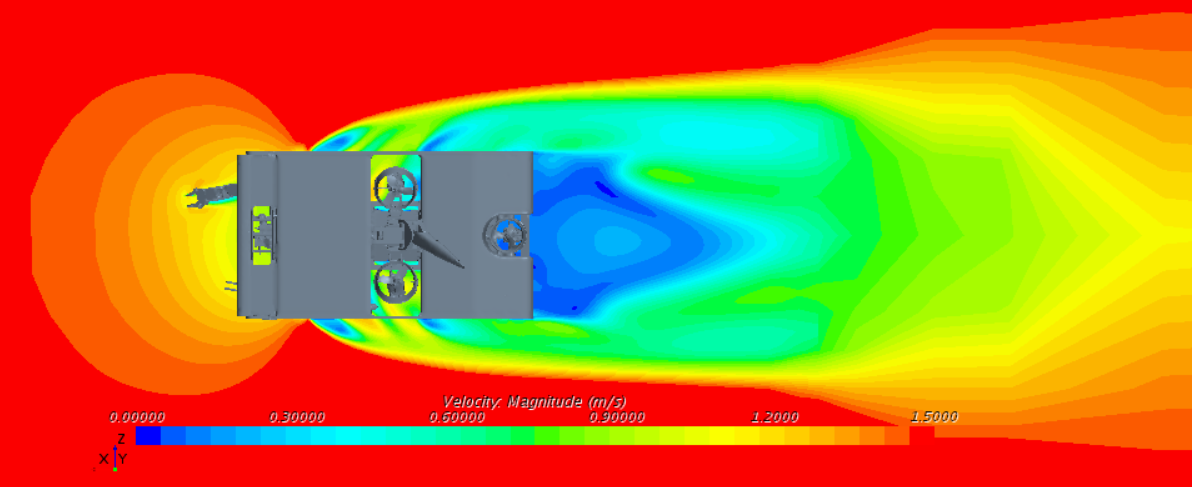
\includegraphics[width = 15cm]{figure/chap4/rov_surge3.png}
}
\subfigure[]{
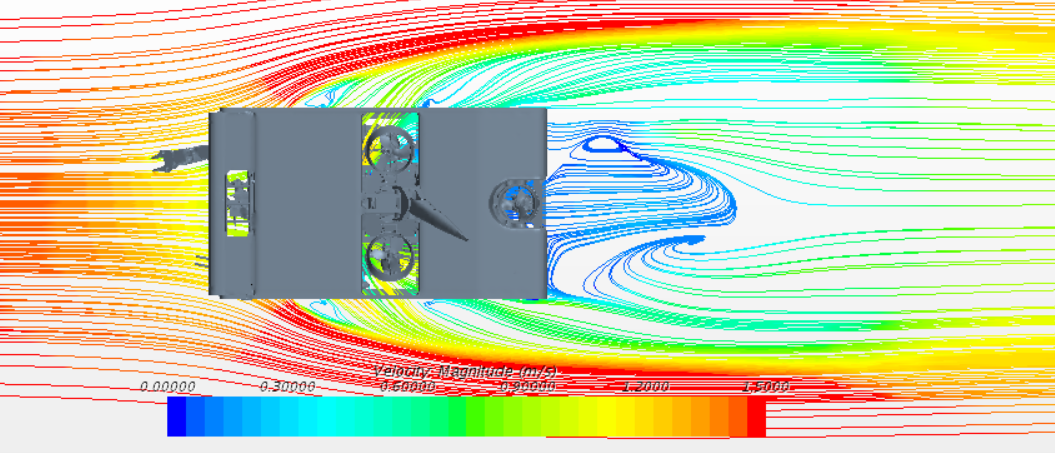
\includegraphics[width = 15cm]{figure/chap4/rov_surge4.png}
}
\bicaption[fig:chap4:F7]{ROV前进速度为1.5m/s时速度流线和矢量图}{ROV前进速度为1.5m/s时速度流线和矢量图}{Fig.}{ Speed streamline and vector diagram for ROV with surge speed 1.5m/s}
\end{figure}


\begin{figure}
\label{fig:chap4:F8}
\centering
\subfigure[]{
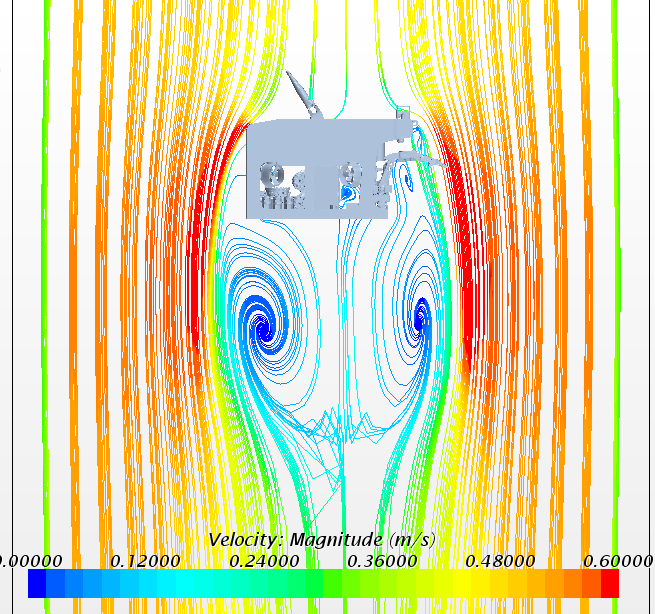
\includegraphics[width = 10cm]{figure/chap4/rov_up1.png}
}
\subfigure[]{
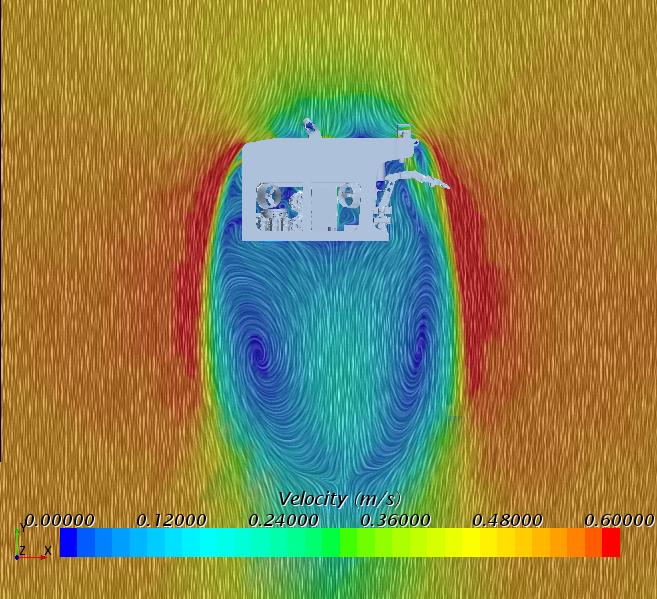
\includegraphics[width = 10cm]{figure/chap4/rov_up2.png}
}
\bicaption[fig:chap4:F8]{ROV上浮速度为0.5m/s时速度流线和矢量图}{ROV上浮速度为0.5m/s时速度流线和矢量图}{Fig.}{ Speed streamline and vector diagram for ROV with floating speed 0.5m/s}
\end{figure}


\begin{figure}
\label{fig:chap4:F9}
\centering
\subfigure[]{
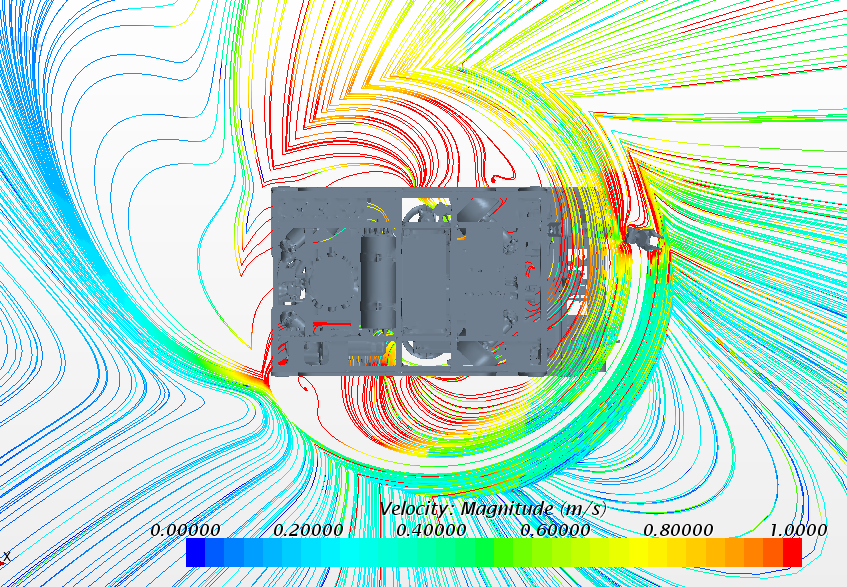
\includegraphics[width = 10cm]{figure/chap4/rov_yaw1.png}
}
\subfigure[]{
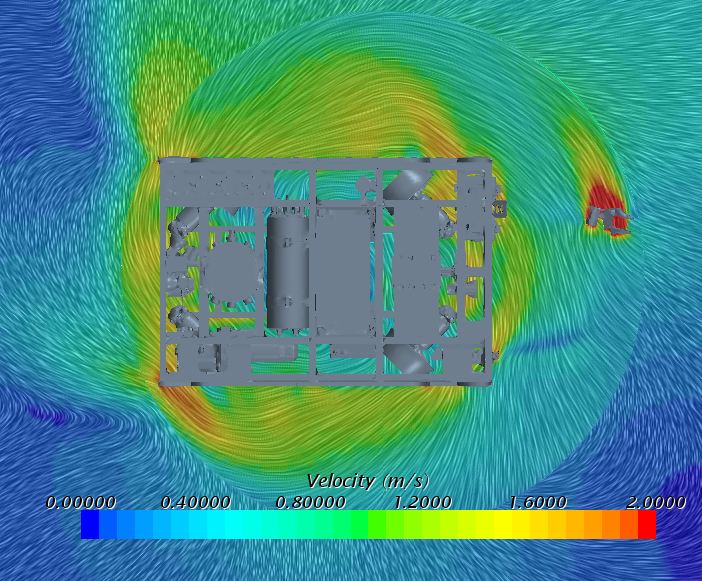
\includegraphics[width = 10cm]{figure/chap4/rov_yaw2.png}
}
\bicaption[fig:chap4:F9]{ROV偏航速度为1.5rad/s时速度流线图和矢量图}{ROV偏航速度为1.5rad/s时速度流线图和矢量图}{Fig.}{ Speed streamline and vector diagram for ROV with yaw rate 1.5rad/s}
\end{figure}

\begin{figure}
\label{fig:chap4:F10}
\centering
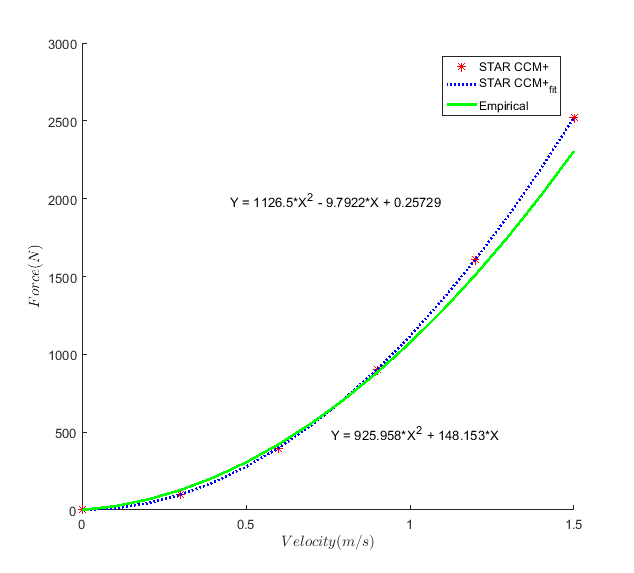
\includegraphics[width = 10cm]{figure/chap4/damping_surge.png}
\bicaption[fig:chap4:F10]{ROV的纵荡自由度的经验法和数值分析拟合结果对比}{ROV的纵荡自由度的经验法和数值分析拟合结果对比}{Fig.}{ Comparision between empirical method and numerical analysis in the ROV's surge channel}
\end{figure}

\begin{figure}
\label{fig:chap4:F11}
\centering
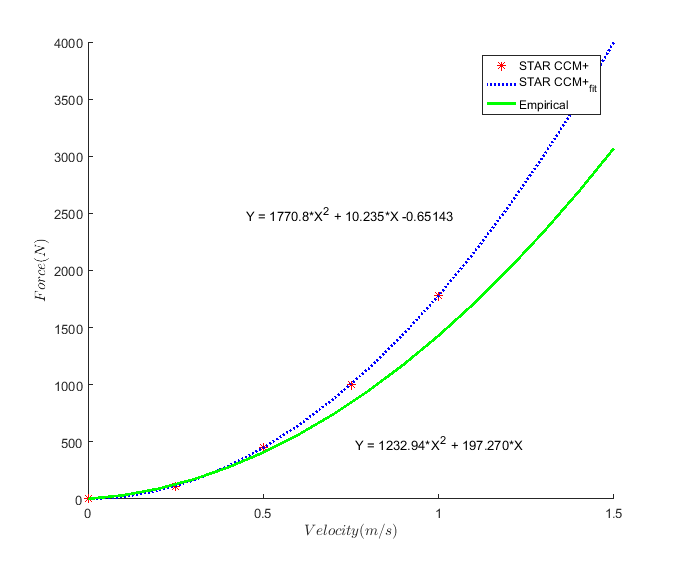
\includegraphics[width = 10cm]{figure/chap4/damping_heave.png}
\bicaption[fig:chap4:F11]{ROV的垂荡自由度的经验法和数值分析拟合结果对比}{ROV的垂荡自由度的经验法和数值分析拟合结果对比}{Fig.}{ Comparision between empirical method and numerical analysis in the ROV's heave channel}
\end{figure}

\begin{figure}
\label{fig:chap4:F12}
\centering
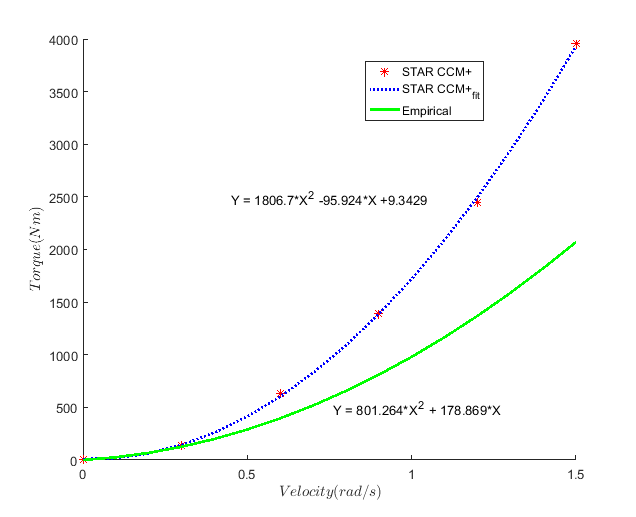
\includegraphics[width = 10cm]{figure/chap4/damping_yaw.png}
\bicaption[fig:chap4:F12]{ROV的偏航自由度的经验法和数值分析拟合结果对比}{ROV的偏航自由度的经验法和数值分析拟合结果对比}{Fig.}{ Comparision between empirical method and numerical analysis in the ROV's yaw channel}
\end{figure}


采用AQWA软件和STAR CCM+软件分别预测附加质量项和阻尼力的估计方程,结果如下:

附加质量:

\begin{equation}
\begin{aligned}
\bm{M_{A}} = \begin{bmatrix}
     877.31 &   5.5756 &  -114.49 &  -1.8992 &   447.47 &   3.9657\\
     4.8538 &   1432.8 &  -1.4758 &  -468.2  &   6.0126 &    361.5\\
     -115.54 &  -5.9954  &  1763  &  -4.8197 &  -693.41 &  -5.3964\\
     -0.78241 &  -490.1  &  -1.8668  &  539.36 & 2.6651  &  -140.62\\
     452.9  &  6.195 &  -694.04  &  3.5358 &   1160.4  & -0.77008\\
     2.4616  &  355.83 &  -3.8789 &  -130.34 &  -0.94418  &  598.42\\
         \end{bmatrix}
\end{aligned}
\end{equation}


将经验法和数值分析方法获得附加质量进行对比,可以发现两者之间存在着一致性。对于阻尼项,通过分析两种不同方法计算的阻尼力预测值对比结果,可以看出虽然经验法和数值计算法两者之间存在一定的差异,但是也在数量级上具有一致性,可以验证本节给出的两种方法的有效性。


\section{基于泰勒公式简化的水下机器人模型建立  }

控制导向的水下机器人建模,在水下机器人数学模型描述未知时,可以采用经验法和数值分析法预测水动力模型参数。然而在有些水下机器人案例中,水下机器人的模型是基于潜艇、鱼雷模型以及舵片经验数据来确定的\cite{yuanchuan2001submarine,Borst1985Fluid,bottaccini1954stablity}。在水下机器人的数学模型描述已知但是却非线性耦合非常严重时,就需要基于控制目标进行数学处理。

经常用于模型参考自适应控制应用中的水下机器人系统模型可以根据系统的模型形式分为线性系统和非线性系统。 然而,大多数模型参考自适应控制中引入的线性系统模型是通过忽略航行器系统中的高阶或非线性项而从实际航行器中推导出来的。通过理论和经验数据相结合的REMUS 100 AUV的6自由度(DOF)非线性系统模型为改善REMUS的控制提供了更精确的航行器平台。

REMUS AUV的非线性模型的高度复杂性,对于后续的控制带来了很大挑战。 REMUS AUV模型是总结实验数据而建立的非线性模型,它对于研究AUV的动力学的性能和控制器设计都非常重要,但是由于其建立是从动力学分析角度建立的,并不完全适用于控制应用。AUV水下机器人多是由舵片和推进器共同驱动,但由于舵片本身的工作空间受限制,且该类型的水下机器人多是欠驱动的,因此在进行位置和姿态控制的时候,仅仅选择其中几个关键量进行控制。

本节选择以控制俯仰姿态为目标,从水下机器人的6自由度运动动力学模型中提取出俯仰姿态的控制方程:
\begin{equation}
\label{depth_equ}
\begin{array}{l}
 z =  - {\rm{sin}}\theta u + \cos \theta \sin \varphi v + \cos \theta \cos \varphi \omega  \\
 {I_y}\dot q + ({I_x} - {I_z})rp + m[{z_G}(\dot u - vr + \omega q) - {x_G}(\dot \omega  - uq + vp)] =  - ({z_G}W - {z_B}B)\sin \theta  \\
 \begin{array}{*{20}{c}}
   {} & {}  \\
\end{array} - ({x_G}W - {x_B}B)\cos \theta \cos \varphi  + {M_{\omega \left| \omega  \right|}}\omega \left| \omega  \right| + {M_{q\left| q \right|}}q\left| q \right| + {M_{\dot \omega }}\dot \omega  + M_{\dot q}^{}q + {M_{uq}}uq \\
 \begin{array}{*{20}{c}}
   {} & {}  \\
\end{array} + {M_{vp}}vp + {M_{rp}}rp + {M_{u\omega }}u\omega  + {M_{uu\delta }}{u^2}{\delta _e} \\
 \theta  = \cos \varphi q - \sin \varphi r \\
 \end{array}
\end{equation}
其中 $\delta_e$ 是水平舵片输入角。

为了获得控制用的方程,方程可以在操作点$\theta_0$, $q_0$, $u_0$, $z_0$ 使用泰勒公式进行展开,并忽略其中的高阶项,则可以得到简化后的模型如下:

\begin{equation}
\begin{array}{l}
 z =  - {u_0}\cos {\theta _0}\theta  \\
 {I_y}\dot q + m{x_G}{u_0}q =  - ({z_G}W - {z_B}B)\cos {\theta _0}\theta  \\
 \begin{array}{*{20}{c}}
   {\begin{array}{*{20}{c}}
   {} & {}  \\
\end{array}}  \\
\end{array} + ({x_G}W - {x_B}B)\sin {\theta _0}\theta  + 2{M_{\left| q \right|q}}\left| {{q_0}} \right|q \\
 \begin{array}{*{20}{c}}
   {\begin{array}{*{20}{c}}
   {} & {}  \\
\end{array}}  \\
\end{array} + {M_{\dot q}}\dot q + {M_{uq}}{u_0}q + {M_{uu\delta }}u_0^2{\delta _e} \\
 \dot \theta  = q \\
 \end{array}
\end{equation}

简化后的方程被转为带有不确定性的状态方程的形式:

\begin{equation}
\begin{array}{l}
 \left[ {\begin{array}{*{20}{c}}
   {\dot \theta }  \\
   {\dot q}  \\
\end{array}} \right] = \left[ {\begin{array}{*{20}{c}}
   0 & 1  \\
   {\frac{{ - ({z_G}W - {z_B}B)\cos {\theta _0}}}{{{I_y} - {M_{\dot q}}}}} & {\frac{{ - m{x_G}u_0^{} + 2{M_{q\left| q \right|}}\left| {{q_0}} \right| + {M_{uq}}{u_0}}}{{{I_y} - {M_{\dot q}}}}}  \\
\end{array}} \right]\left[ {\begin{array}{*{20}{c}}
   \theta   \\
   q  \\
\end{array}} \right] + \left[ {\begin{array}{*{20}{c}}
   0  \\
   {\frac{{{M_{uu\delta }}{u_0}^2}}{{{I_y} - {M_{\dot q}}}}}  \\
\end{array}} \right]{\delta _e} \\
 \begin{array}{*{20}{c}}
   {} & { + \frac{1}{{{I_y} - {M_{\dot q}}}}\left[ {\begin{array}{*{20}{c}}
   0 & 0 & 0  \\
   \gamma  & \lambda  & \zeta   \\
\end{array}} \right]}  \\
\end{array}\left[ {\begin{array}{*{20}{c}}
   u  \\
   q  \\
   \theta   \\
\end{array}} \right] \\
 \end{array}
\end{equation}
其中, $\gamma$,$\lambda$,$\zeta$ 是与$u$, $q$, $\theta$相关的不确定性系数。此外,横滚自由度的横滚角$\varphi$、速度$p$在方程中是被视为干扰的。

采用本节的非线性模型简化方法,可以获得用于控制的参考模型方程,对于其他的自由度,也可以参考与此类似的方法进行处理。

\section{本章小结 }

本章系统地研究了水下机器人的用于鲁棒自适应控制的建模问题。水下机器人的种类不同,模型确定方法也有差异,用于控制目标的水下机器人建模,不必非常精确,但是应能表征水下机器人所要控制模式的主要部分。本章分别从水下机器人外形、数学模型两个角度对水下机器人进行建模。基于机器人外形而进行的建模主要分为经验法和流体软件数值分析法,以上方法可适用于具有非初等几何外形的ROV,而具有流线型且已知非线性模型的AUV,可以以控制目标为导向对模型进行数学简化,并分析控制模型的不确定性。首先,考虑到水下机器人的模型未知且实验数据不可获取,仅仅具有水下机器人的一些设置功能要求以及物理模型等资料,尤其对于非初等几何表面的低速水下机器人,通过分析水下机器人动力学模型的各个项的重要性,简化动力学模型,并确定了附加质量和非线性阻尼为主要计算项。经验法主要基于实验数据的总结,可以对水动力参数进行相对精确的快速估算。数值分析方法主要使用流体计算软件STAR CCM+和ANSYS/AWQA软件分别求取模型关键参数和提取重要的数据。其次,针对水下机器人非线性精确模型已知,对运动方程进行解耦,并进行泰勒展开,确定可以用于自适应控制的参考模型,本章给出了俯仰模式的泰勒展开模型。本章给出的方法从多个角度为水下机器人进行建模,最大程度了方便了控制应用。
